\documentclass[12pt,a4paper,notitlepage,oneside,amsmath,amssymb]{article}
\usepackage{geometry}  % See geometry.pdf to learn the layout options. There are lots.
\geometry{a4paper, margin=1in, noheadfoot} % ... or a4paper or a5paper or ...
\usepackage[utf8]{inputenc}
\usepackage{graphicx}
\graphicspath{{./img/}}
\usepackage{amsmath}
\usepackage{amssymb}
% \usepackage{fontspec}
% \setromanfont{LiHei Pro}
% \XeTeXlinebreaklocale "zh"
% \XeTeXlinebreakskip = 0pt plus 1pt
\usepackage{CJKutf8}
\usepackage{anyfontsize}
\usepackage{caption}
\usepackage{indentfirst}
\usepackage{titlesec}
\usepackage{enumitem}
\usepackage[normalem]{ulem}
\usepackage[most]{tcolorbox}
% \tcbuselibrary{breakable}
% \usepackage{cancel}
\usepackage{xcolor}
% \usepackage[pages=all]{background}
\definecolor{text}{rgb}{0.1, 0.1, 0.1}
\color{black}

\titleformat*{\section}{\large\bfseries}
\titleformat*{\subsection}{\large\bfseries}
\titleformat*{\subsubsection}{\large\bfseries}
\titleformat*{\paragraph}{\large\bfseries}
\titleformat*{\subparagraph}{\large\bfseries}
% \titlespacing*{<command>}{<left>}{<before-sep>}{<after-sep>}
\titlespacing*{\section}{0pt}{15pt}{4pt}


% \setlength{\parindent}{0em}
% \setlength{\parskip}{0.5em}
% \setlength{\columnsep}{0.5cm}
\renewcommand{\baselinestretch}{1.2} % scales the default interline space to 1.5 its default value.

\setlist[itemize]{topsep=2pt, itemsep=0.2ex, partopsep=0ex, parsep=0ex, nosep, leftmargin=3ex,
labelindent=1ex, labelwidth=1ex}
% \setlist[enumerate]{topsep=2pt, itemsep=0.2ex, partopsep=0.5ex, parsep=0.2ex, nosep,
%     labelindent=2ex, labelwidth=2ex}

\begin{document}
\begin{CJK*}{UTF8}{bkai}

  \CJKtilde{}
  \CJKindent{}
  \title{\vspace{-10ex}DIP HW1 Report}
  \author{R07922036~邱能賢}
  \date{\vspace{-1ex}\today}

  \maketitle

  \vspace{-5ex}

  \section*{Warm-up: Simple Manipulations}
  \begin{enumerate}[label=(\alph*)]
    \item Perform horizontal flipping on image \(I_1\).

          To flip the image horizontally, I created a new image array and fill in each row of pixels in reverse order.
          \begin{figure}[hbt!]
            \begin{minipage}{.5\textwidth}
              \centering
              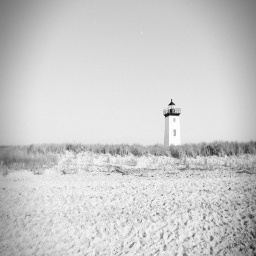
\includegraphics[width=.6\linewidth]{sample1}
              \caption{\(I_1\), sample1.raw}
              \label{fig:sample1}
            \end{minipage}%
            \begin{minipage}{.5\textwidth}
              \centering
              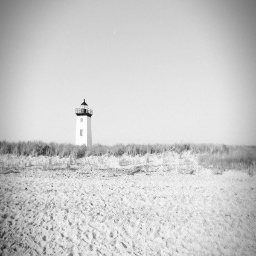
\includegraphics[width=.6\linewidth]{imageB}
              \caption{image \(B\)}
              \label{fig:imageB}
            \end{minipage}
          \end{figure}
    \item Perform a power-law transform to enhance image $B$.

          The following are the transformed images with their corresponding histograms using different transform functions. As the power goes larger, the image becomes darker and the contrast increases. But the sky becomes more noisy in the image with power = 3.
          \begin{figure}[hbt!]
            \begin{minipage}{.25\textwidth}
              \centering
              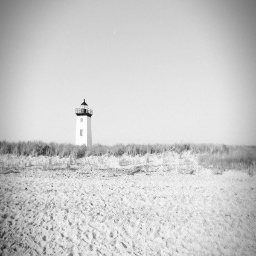
\includegraphics[width=.95\linewidth]{imageB}
            \end{minipage}%
            \begin{minipage}{.25\textwidth}
              \centering
              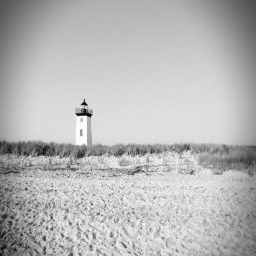
\includegraphics[width=.95\linewidth]{imageC-1_5}
            \end{minipage}%
            \begin{minipage}{.25\textwidth}
              \centering
              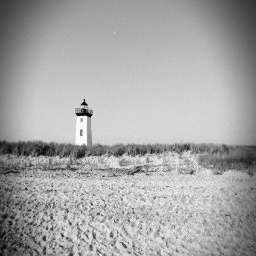
\includegraphics[width=.95\linewidth]{imageC-2}
            \end{minipage}%
            \begin{minipage}{.25\textwidth}
              \centering
              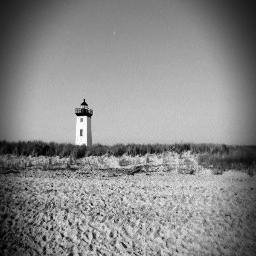
\includegraphics[width=.95\linewidth]{imageC-3}
            \end{minipage}
            \begin{minipage}{.25\textwidth}
              \centering
              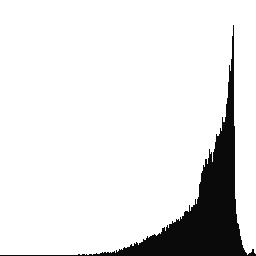
\includegraphics[width=.95\linewidth]{imageB_hist}
              \caption*{image \(B\)}
            \end{minipage}%
            \begin{minipage}{.25\textwidth}
              \centering
              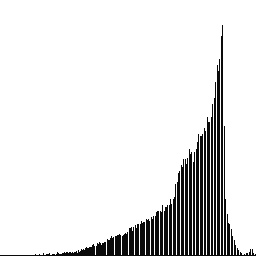
\includegraphics[width=.95\linewidth]{imageC-1_5_hist}
              \caption*{Power \(= 1.5\)}
            \end{minipage}%
            \begin{minipage}{.25\textwidth}
              \centering
              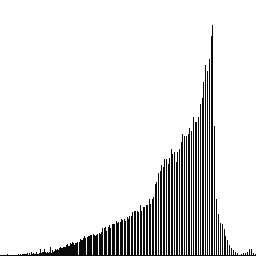
\includegraphics[width=.95\linewidth]{imageC-2_hist}
              \caption*{Power \(= 2.0\)}
            \end{minipage}%
            \begin{minipage}{.25\textwidth}
              \centering
              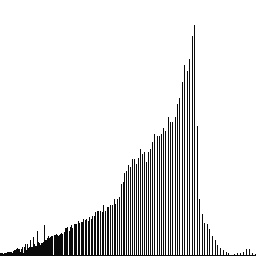
\includegraphics[width=.95\linewidth]{imageC-3_hist}
              \caption*{Power \(= 3.0\)}
            \end{minipage}
          \end{figure}
  \end{enumerate}

  \section*{Problem 1: Image Enhancement}
  \begin{enumerate}[label=(\alph*)]
    \item Decrease the brightness of \(I_2\) by dividing the intensity values by 2 as image \(D\).
    \item Decrease the brightness of \(I_2\) by dividing the intensity values by 3 as image \(E\).

          \begin{figure}[hbt!]
            \centering
            \begin{minipage}{.33\textwidth}
              \centering
              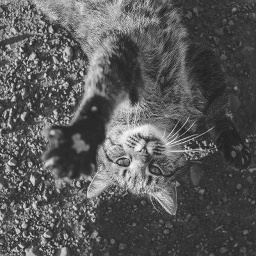
\includegraphics[width=.8\linewidth]{sample2}
              \caption{\(I_2\), sample2.raw}
            \end{minipage}%
            \begin{minipage}{.33\textwidth}
              \centering
              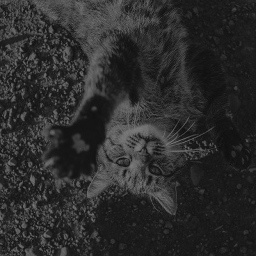
\includegraphics[width=.8\linewidth]{imageD}
              \caption{image \(D\)}
            \end{minipage}%
            \begin{minipage}{.33\textwidth}
              \centering
              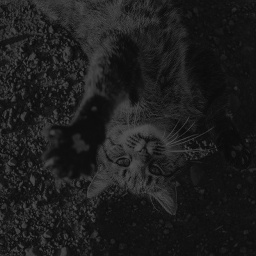
\includegraphics[width=.8\linewidth]{imageE}
              \caption{image \(E\)}
            \end{minipage}
          \end{figure}

    \item Plot the histograms of \(I_2\), \(D\) and \(E\).

          With the intensity divided, the images become much darker and the contrast is very low. From the histogram we can see that for image \(E\), the intensity is limited to the lower \(1/3\).

          \begin{figure}[hbt!]
            \centering
            \begin{minipage}{.33\textwidth}
              \centering
              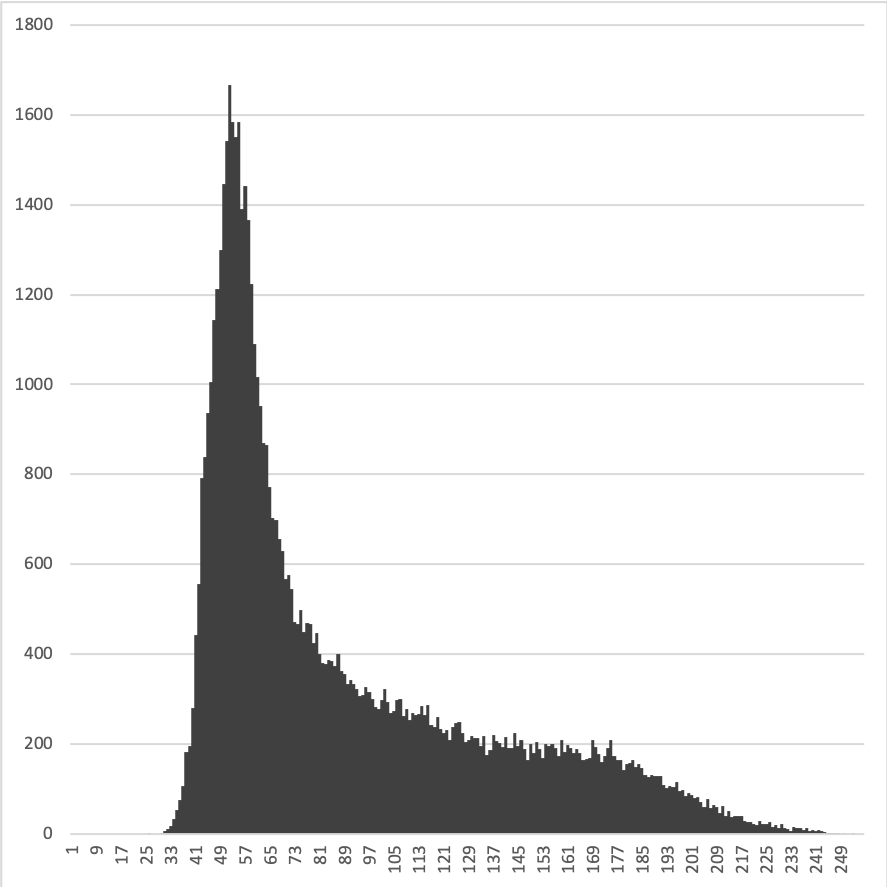
\includegraphics[width=.8\linewidth]{hist_I2}
              \caption*{Histogram of \(I_2\)}
            \end{minipage}%
            \begin{minipage}{.33\textwidth}
              \centering
              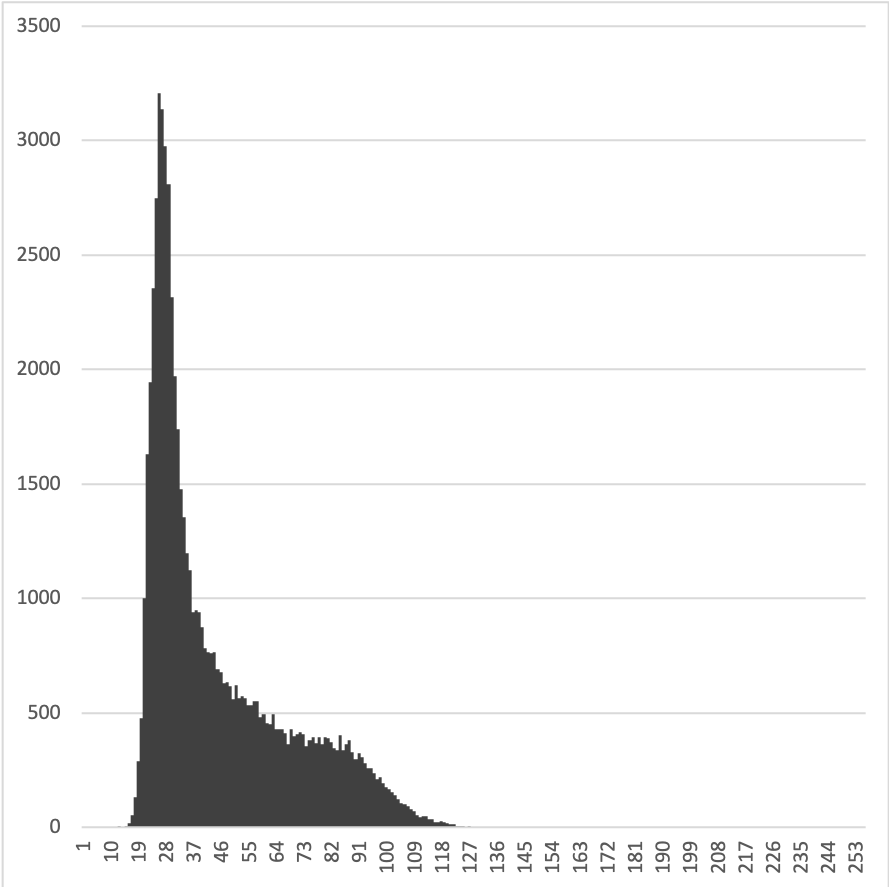
\includegraphics[width=.8\linewidth]{hist_D}
              \caption*{Histogram of image \(D\)}
            \end{minipage}%
            \begin{minipage}{.33\textwidth}
              \centering
              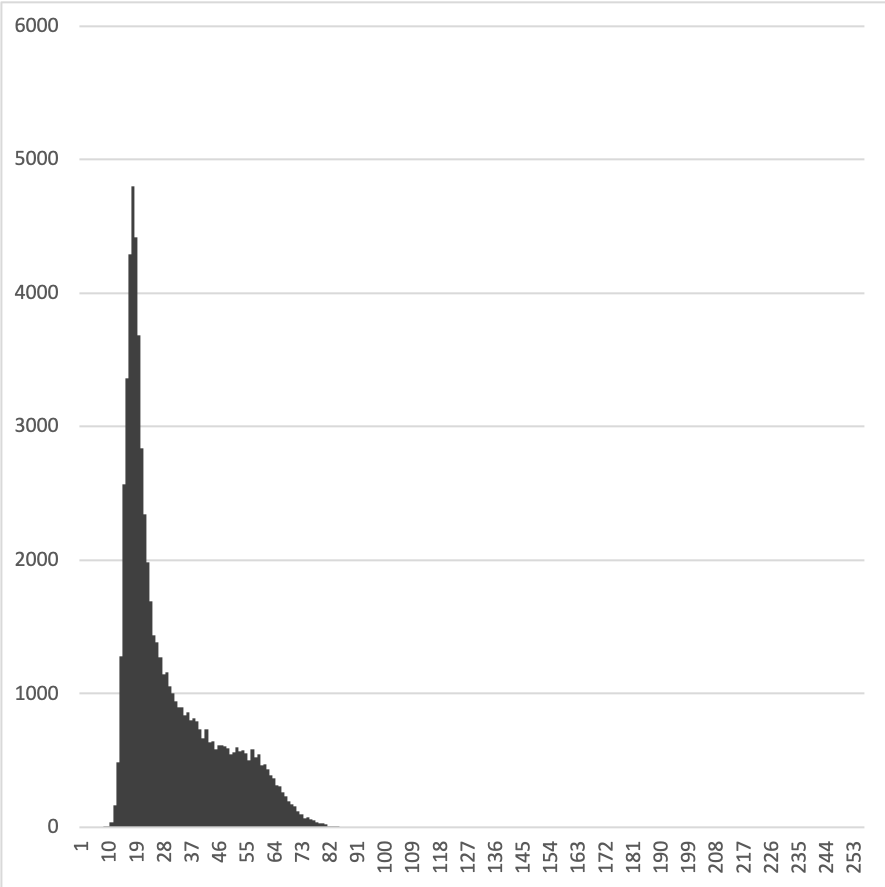
\includegraphics[width=.8\linewidth]{hist_E}
              \caption*{Histogram of image \(E\)}
            \end{minipage}
          \end{figure}


          \newpage
    \item Perform global histogram equalization on \(D\) and \(E\) and output the results as \(H_D\) and \(H_E\) respectively.

          I cannot see clear difference directly between image \(H_D\) and \(H_E\), but although the histograms of \(H_D\) and \(H_E\) have roughly the same shape (due to histogram equalization), the distribution of \(H_E\) is sparser. Because the intensity of image \(E\) is compressed to a smaller range, their are more lost information, so some pixels cannot be distinguished when doing histogram equalization.

          \begin{figure}[hbt!]
            \centering
            \begin{minipage}{.25\textwidth}
              \centering
              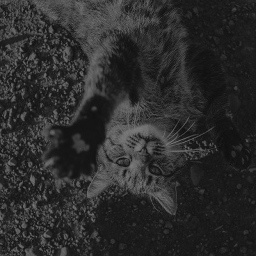
\includegraphics[width=.95\linewidth]{imageD}
              \caption*{image \(D\)}
            \end{minipage}%
            \begin{minipage}{.25\textwidth}
              \centering
              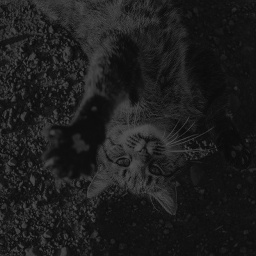
\includegraphics[width=.95\linewidth]{imageE}
              \caption*{image \(E\)}
            \end{minipage}%
            \begin{minipage}{.25\textwidth}
              \centering
              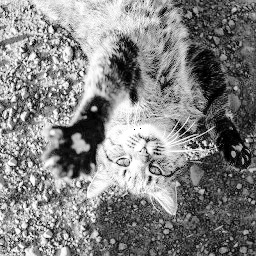
\includegraphics[width=.95\linewidth]{image_HD}
              \caption*{image \(H_D\)}
            \end{minipage}%
            \begin{minipage}{.25\textwidth}
              \centering
              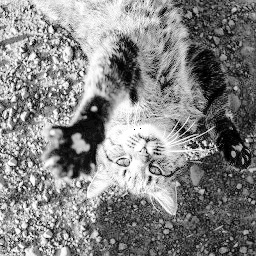
\includegraphics[width=.95\linewidth]{image_HE}
              \caption*{image \(H_E\)}
            \end{minipage}
            \begin{minipage}{.25\textwidth}
              \centering
              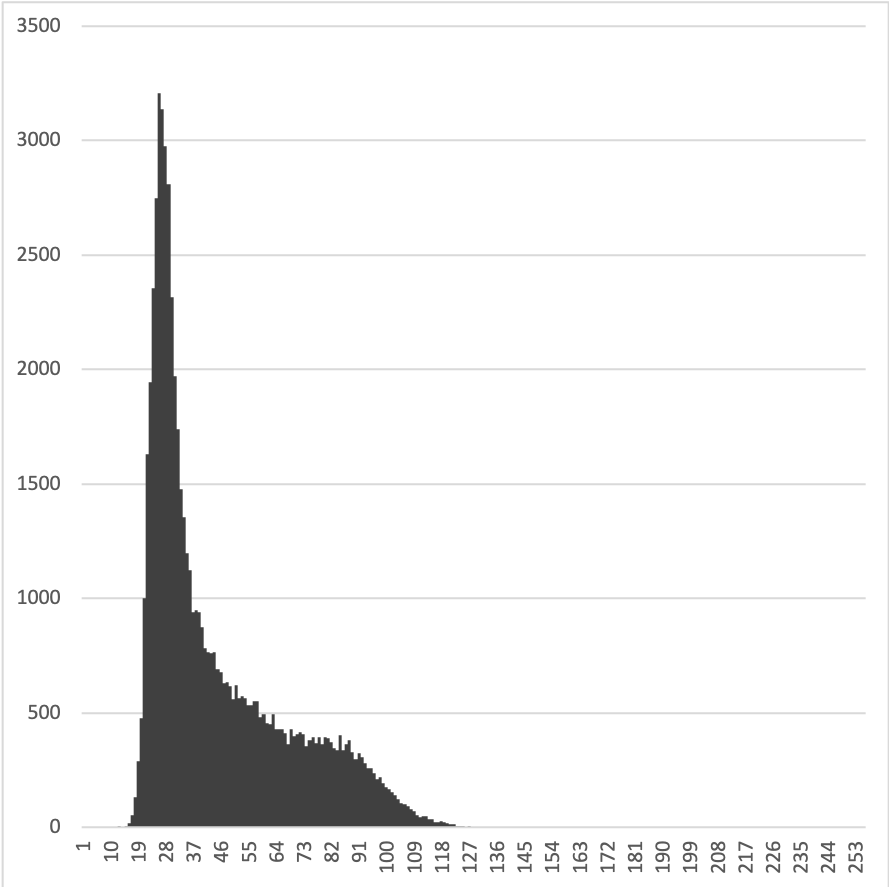
\includegraphics[width=.95\linewidth]{hist_D}
              \caption*{Histogram of \(D\)}
            \end{minipage}%
            \begin{minipage}{.25\textwidth}
              \centering
              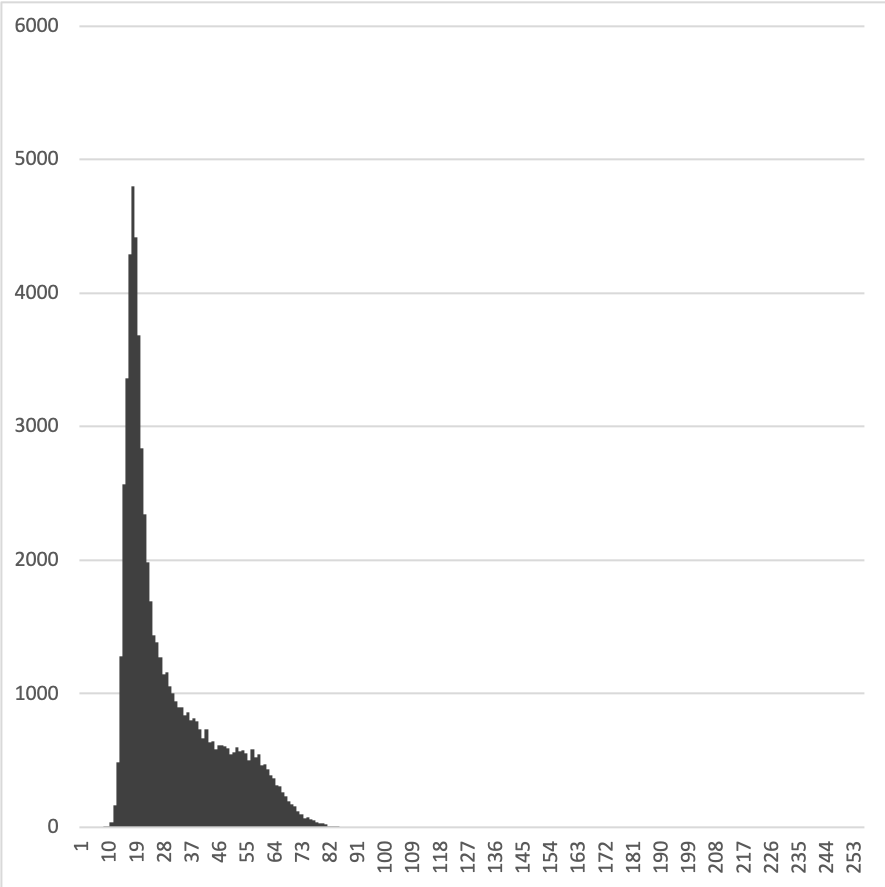
\includegraphics[width=.95\linewidth]{hist_E}
              \caption*{Histogram of \(E\)}
            \end{minipage}%
            \begin{minipage}{.25\textwidth}
              \centering
              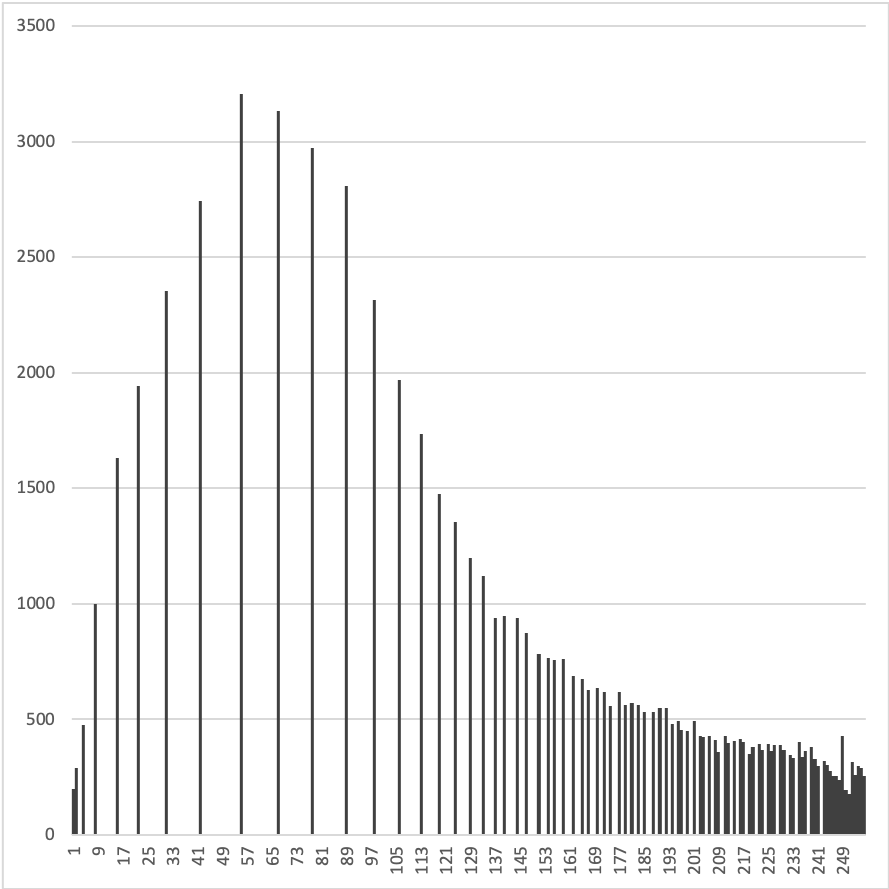
\includegraphics[width=.95\linewidth]{hist_HD}
              \caption*{Histogram of \(H_D\)}
            \end{minipage}%
            \begin{minipage}{.25\textwidth}
              \centering
              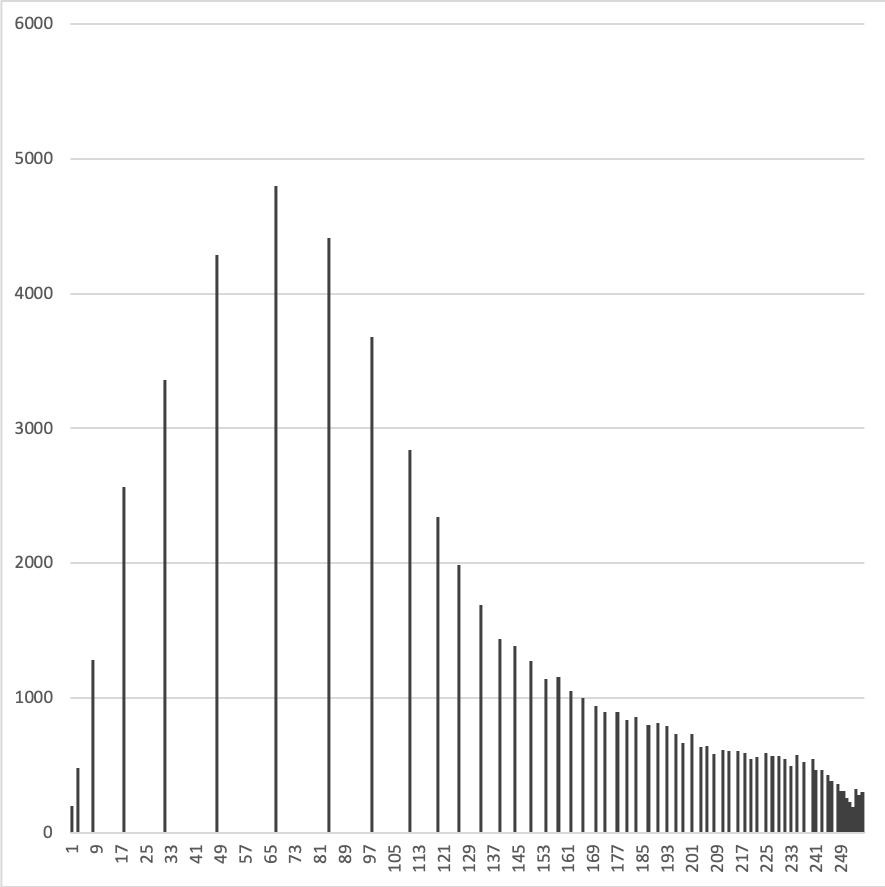
\includegraphics[width=.95\linewidth]{hist_HE}
              \caption*{Histogram of \(H_E\)}
            \end{minipage}
          \end{figure}

          \newpage
    \item Perform local histogram equalization on \(D\) and \(E\) and output the results as \(L_D\) and \(L_E\) respectively.

          Local histogram equalization is done on each pixel with a transformation function derived from a neighboring \(32 \times 32\) block and apply histogram equalization. At the image boundaries, the block is sampled by mirroring pixels with respect to the boundary.

          Because the transformation function of each pixel is derived individually, there are no gaps in the histograms as those of global histogram equalization.

          \begin{figure}[hbt!]
            \centering
            \begin{minipage}{.25\textwidth}
              \centering
              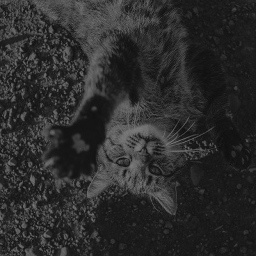
\includegraphics[width=.95\linewidth]{imageD}
              \caption*{image \(D\)}
            \end{minipage}%
            \begin{minipage}{.25\textwidth}
              \centering
              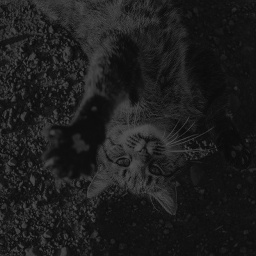
\includegraphics[width=.95\linewidth]{imageE}
              \caption*{image \(E\)}
            \end{minipage}%
            \begin{minipage}{.25\textwidth}
              \centering
              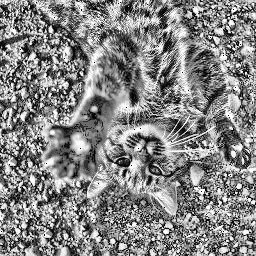
\includegraphics[width=.95\linewidth]{image_LD}
              \caption*{image \(L_D\)}
            \end{minipage}%
            \begin{minipage}{.25\textwidth}
              \centering
              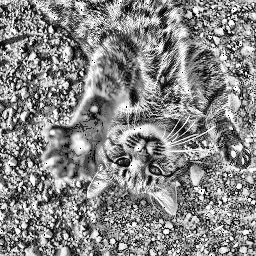
\includegraphics[width=.95\linewidth]{image_LE}
              \caption*{image \(L_E\)}
            \end{minipage}
            \begin{minipage}{.25\textwidth}
              \centering
              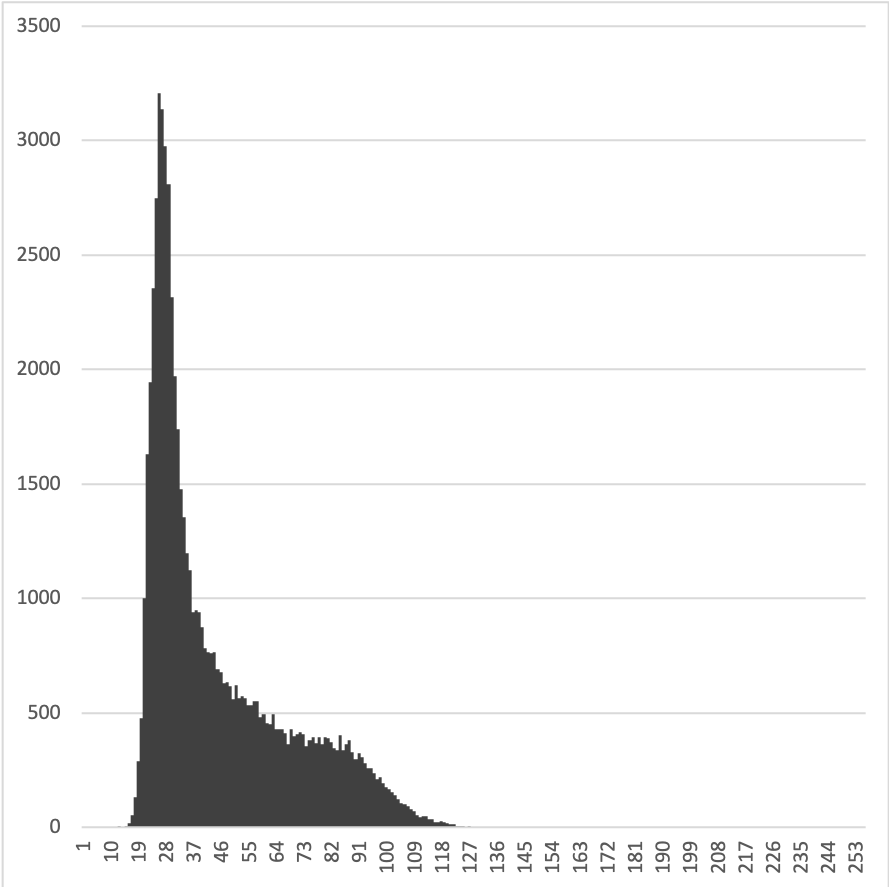
\includegraphics[width=.95\linewidth]{hist_D}
              \caption*{Histogram of \(D\)}
            \end{minipage}%
            \begin{minipage}{.25\textwidth}
              \centering
              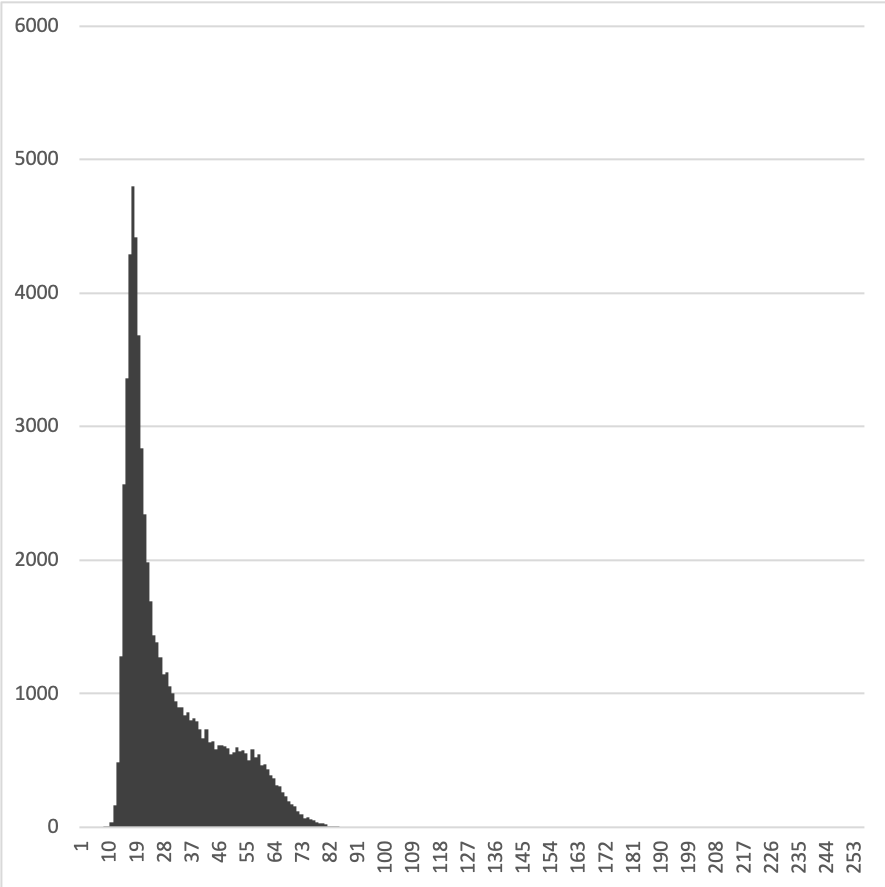
\includegraphics[width=.95\linewidth]{hist_E}
              \caption*{Histogram of \(E\)}
            \end{minipage}%
            \begin{minipage}{.25\textwidth}
              \centering
              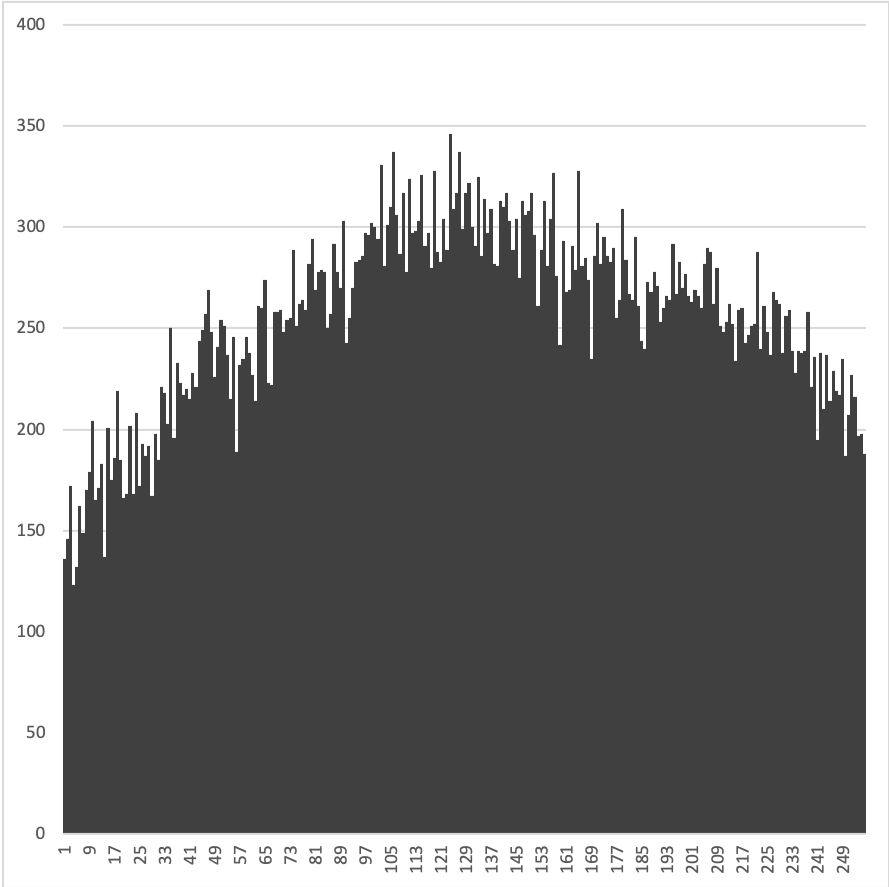
\includegraphics[width=.95\linewidth]{hist_LD}
              \caption*{Histogram of \(L_D\)}
            \end{minipage}%
            \begin{minipage}{.25\textwidth}
              \centering
              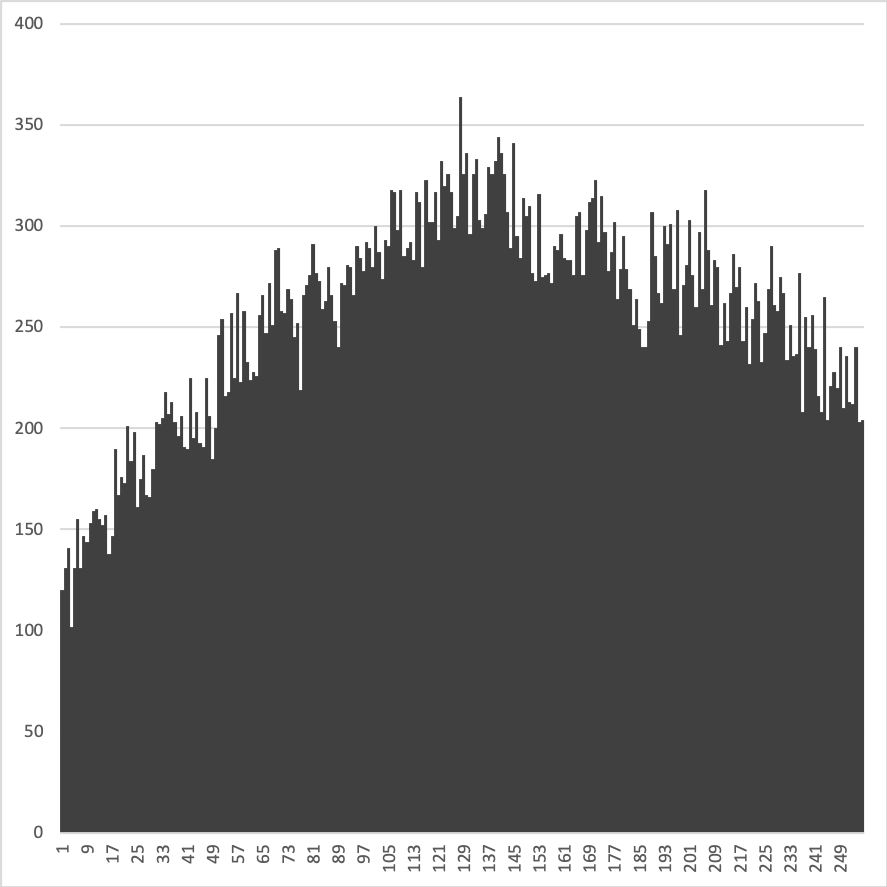
\includegraphics[width=.95\linewidth]{hist_LE}
              \caption*{Histogram of \(L_E\)}
            \end{minipage}
          \end{figure}

    \item Comparing local histogram equalization to global histogram equalization, the contrast of each region is more enhanced and also more uniform throughout the image. The histograms are also more uniformly distributed.
  \end{enumerate}

  \section*{Problem 2: Noise Removal}
  \begin{enumerate}[label=(\alph*)]
    \item Remove noise from Fig.3(b) and Fig.3(c).

          \begin{figure}[hbt!]
            \centering
            \begin{minipage}{.25\textwidth}
              \centering
              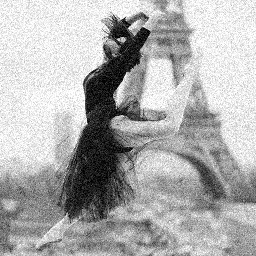
\includegraphics[width=.97\linewidth]{sample4}
              \caption*{Fig.3(b)}
            \end{minipage}%
            \begin{minipage}{.25\textwidth}
              \centering
              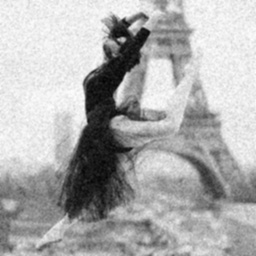
\includegraphics[width=.97\linewidth]{imageN1}
              \caption*{image \(N_1\)}
            \end{minipage}%
            \begin{minipage}{.25\textwidth}
              \centering
              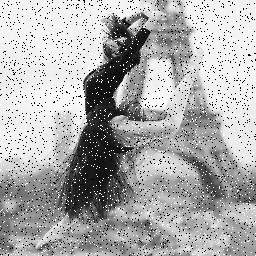
\includegraphics[width=.97\linewidth]{sample5}
              \caption*{Fig.3(c)}
            \end{minipage}%
            \begin{minipage}{.25\textwidth}
              \centering
              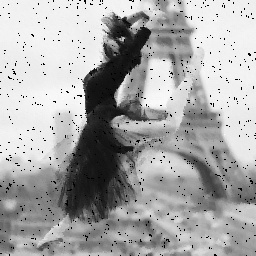
\includegraphics[width=.97\linewidth]{imageN2}
              \caption*{image \(N_2\)}
            \end{minipage}
          \end{figure}

          The noise in Fig.3(b) is more like a uniform noise, so I choose to use low pass filtering to cancel the noise. The filter I used is
          \[
            H = \frac{1}{16}
            \begin{bmatrix}
              1 & 2 & 1 \\
              2 & 4 & 2 \\
              1 & 2 & 1
            \end{bmatrix}
          \]
          The noise in Fig.3(c) is more like a impulse noise, so I choose to use median filtering to cancel the noise.
          Each pixel is set to the median value of the neighboring \(3 \times 3\) block.

    \item Compute the PSNR values of \(N_1\) and \(N_2\). The following is the PSNR of each image.

          \vspace{0.5ex}

          \begin{tabular}{ l | l }
            Fig.3(b) (sample4) & 23.49 \\
            \hline
            image \(N_1\)      & 28.66 \\
            \hline\hline
            Fig.3(c) (sample5) & 14.71 \\
            \hline
            image \(N_2\)      & 18.57
          \end{tabular}

          After the filtering, the PSNR value increased for both Fig.3(b) and Fig.3(C), so the filtering did successfully cancelled out some noise.

  \end{enumerate}

  \clearpage
\end{CJK*}
\end{document}
